\documentclass[8pt,aspectratio=169]{beamer}
%======================================%
\usepackage{times}
\usepackage{amsmath}
\usepackage{amsfonts}
\usepackage{amssymb}
%\usepackage{bm}
\usepackage{newtxtext}
\usepackage[utf8]{inputenc}
\usepackage{enumitem}
\usepackage[T1]{fontenc}
\usepackage{array,multirow}
\usepackage{graphicx}
\usepackage{lmodern}
\usepackage{physics}
\usepackage{tikz}
\usetikzlibrary{fadings}
\newcommand{\bd}[1]{\textbf{#1}}
% package for emumerate(not comaptible with beamer) and itemize
\usepackage{pifont}
%package for text Boxes
%==================================%
%fbox preamble
\renewcommand\fbox{\fcolorbox{blue}{orange!20}}
%===================================================%
\usepackage{fancybox}

%==========================================%
% preamble for figure
\usepackage{wrapfig}
\usepackage{blindtext}
%%package for wrap figure around text
\usepackage{subcaption} 
%%package for adding more than one figure
%%package for animation
\usepackage{animate}
%=================color theme==========================%




%===================Font theme=========================%
\setbeamerfont{title}{size=\Large, series=\bfseries, family=\sffamily}
\setbeamerfont{frametitle}{size=\large, series=\bfseries, family=\sffamily}
\setbeamerfont{normal text}{size=\normalsize, family=\sffamily}
%================Frame title customization=============%
\makeatletter
\defbeamertemplate*{frametitle}{mytheme}{	
	\begin{beamercolorbox}[wd=\textwidth,ht=5.5ex,dp=2.25ex]
		{frametitle}{\insertframetitle}
		\centering		
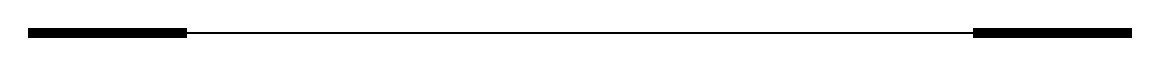
\begin{tikzpicture}
	\draw[black,thick] (0,0)--(12,0);
	%\draw (0,0) rectangle (-2,-0.2);
	\fill[black, draw=black,thick] (0,0) rectangle (-2,0.05) ;
\fill[black, draw=black,thick] (0,0) rectangle (-2,-0.05) ;
	\fill[black, draw=black,thick] (12,0) rectangle (10,0.05) ;
	\fill[black, draw=black,thick] (12,0) rectangle (10,-0.05) ;
\end{tikzpicture}
	\end{beamercolorbox}
}
\makeatother
%------------frame title color and font---------------%
\setbeamercolor{frametitle}{fg=blue}
\setbeamerfont{frametitle}{series=\bfseries,size=\large}
%==========frame page background with gradient===========%
\defbeamertemplate*{background}{mybackground}{
	
\begin{tikzpicture}
		\shade[top color=blue!15, bottom color=white] (0,0) rectangle (\paperwidth,\paperheight);
	\end{tikzpicture}
}
%=============title Page=============================%
\title{\textcolor{black}{Beamer Template}}
\subtitle{\textcolor{black}{Add subtitle }}
\author{Neha Kumari}
\institute{IIT Delhi}
\date{}
\begin{document}
	% frame for title page
{
    \setbeamertemplate{background}
    {
    
\includegraphics[width=\paperwidth,height=\paperheight]{ocean5.jpg}} \begin{frame} 
    \maketitle 	 
 \end{frame}
}
% Presenatation start
\begin{frame}
	\frametitle{Presentation Overview}

	
	
\end{frame}
% Frame for the columns
\begin{frame}{Columns}
% columns with top allignment use [T], for center alignment[c],for bottom alignment[b]
\begin{columns}[T]
	%column 1
	\begin{column}{0.49\textwidth}
	\small	\blindtext
	\end{column}
%column for the verticle length
\begin{column}{0.01\textwidth}
	\rule{0.1mm}{0.7\textheight}
\end{column}
% column 2
	\begin{column}{0.49\textwidth}
		\small	\blindtext
	\end{column}
\end{columns}
\end{frame}
% Frame for the Blocks
\begin{frame}{Blocks}
	% Generic and standard Block
	\begin{block}{Block title}
		block 1
	\end{block}
%Block for the definition
\begin{definition}
	definition
\end{definition}
\end{frame}
% Frame for making table
\begin{frame}
	% begin the lable l= left align, c=ceter align, r=right align
\begin{table}[ht]
	\caption{ Table template}
	\label{tab:table}
	{\tiny	
	\begin{tabular}{|c|c|c|} 
		    \hline
			1&2& 3 \\
			\hline
			4&5&6\\
			\hline
	\end{tabular}
}
\end{table}
\end{frame}
\begin{frame}{wraptable}
	\begin{wraptable}{r}{0.5\textwidth}
		\centering
	\begin{tabular}{|c|c|c|} 
		\hline
		1&2& 3 \\
		\hline
		4&5&6\\
		\hline
	\end{tabular}
\caption{ Table template}
\label{tab:table}
\end{wraptable}
\blindtext
\end{frame}
\begin{frame}{text Boxes}
\shadowbox{Text}\\	
\fbox{text}	\\
\doublebox{text}\\
\ovalbox{text}\\
\end{frame}
\begin{frame}{Lists in Beamer}
\begin{itemize}
	\item[\ding{51}] code 51 
	\item[\ding{56}] code 56
	\item[\ding{43}] code 43
	\item[\ding{45}] code 45
	\item[\ding{79}] code 79
	\item[\ding{118}] code 118
\end{itemize}
\end{frame}
\begin{frame}{figure and column}
\begin{columns}[t]
\begin{column}{0.5\textwidth}
	\blindtext
\end{column}
\begin{column}{0.5\textwidth}
\begin{figure}
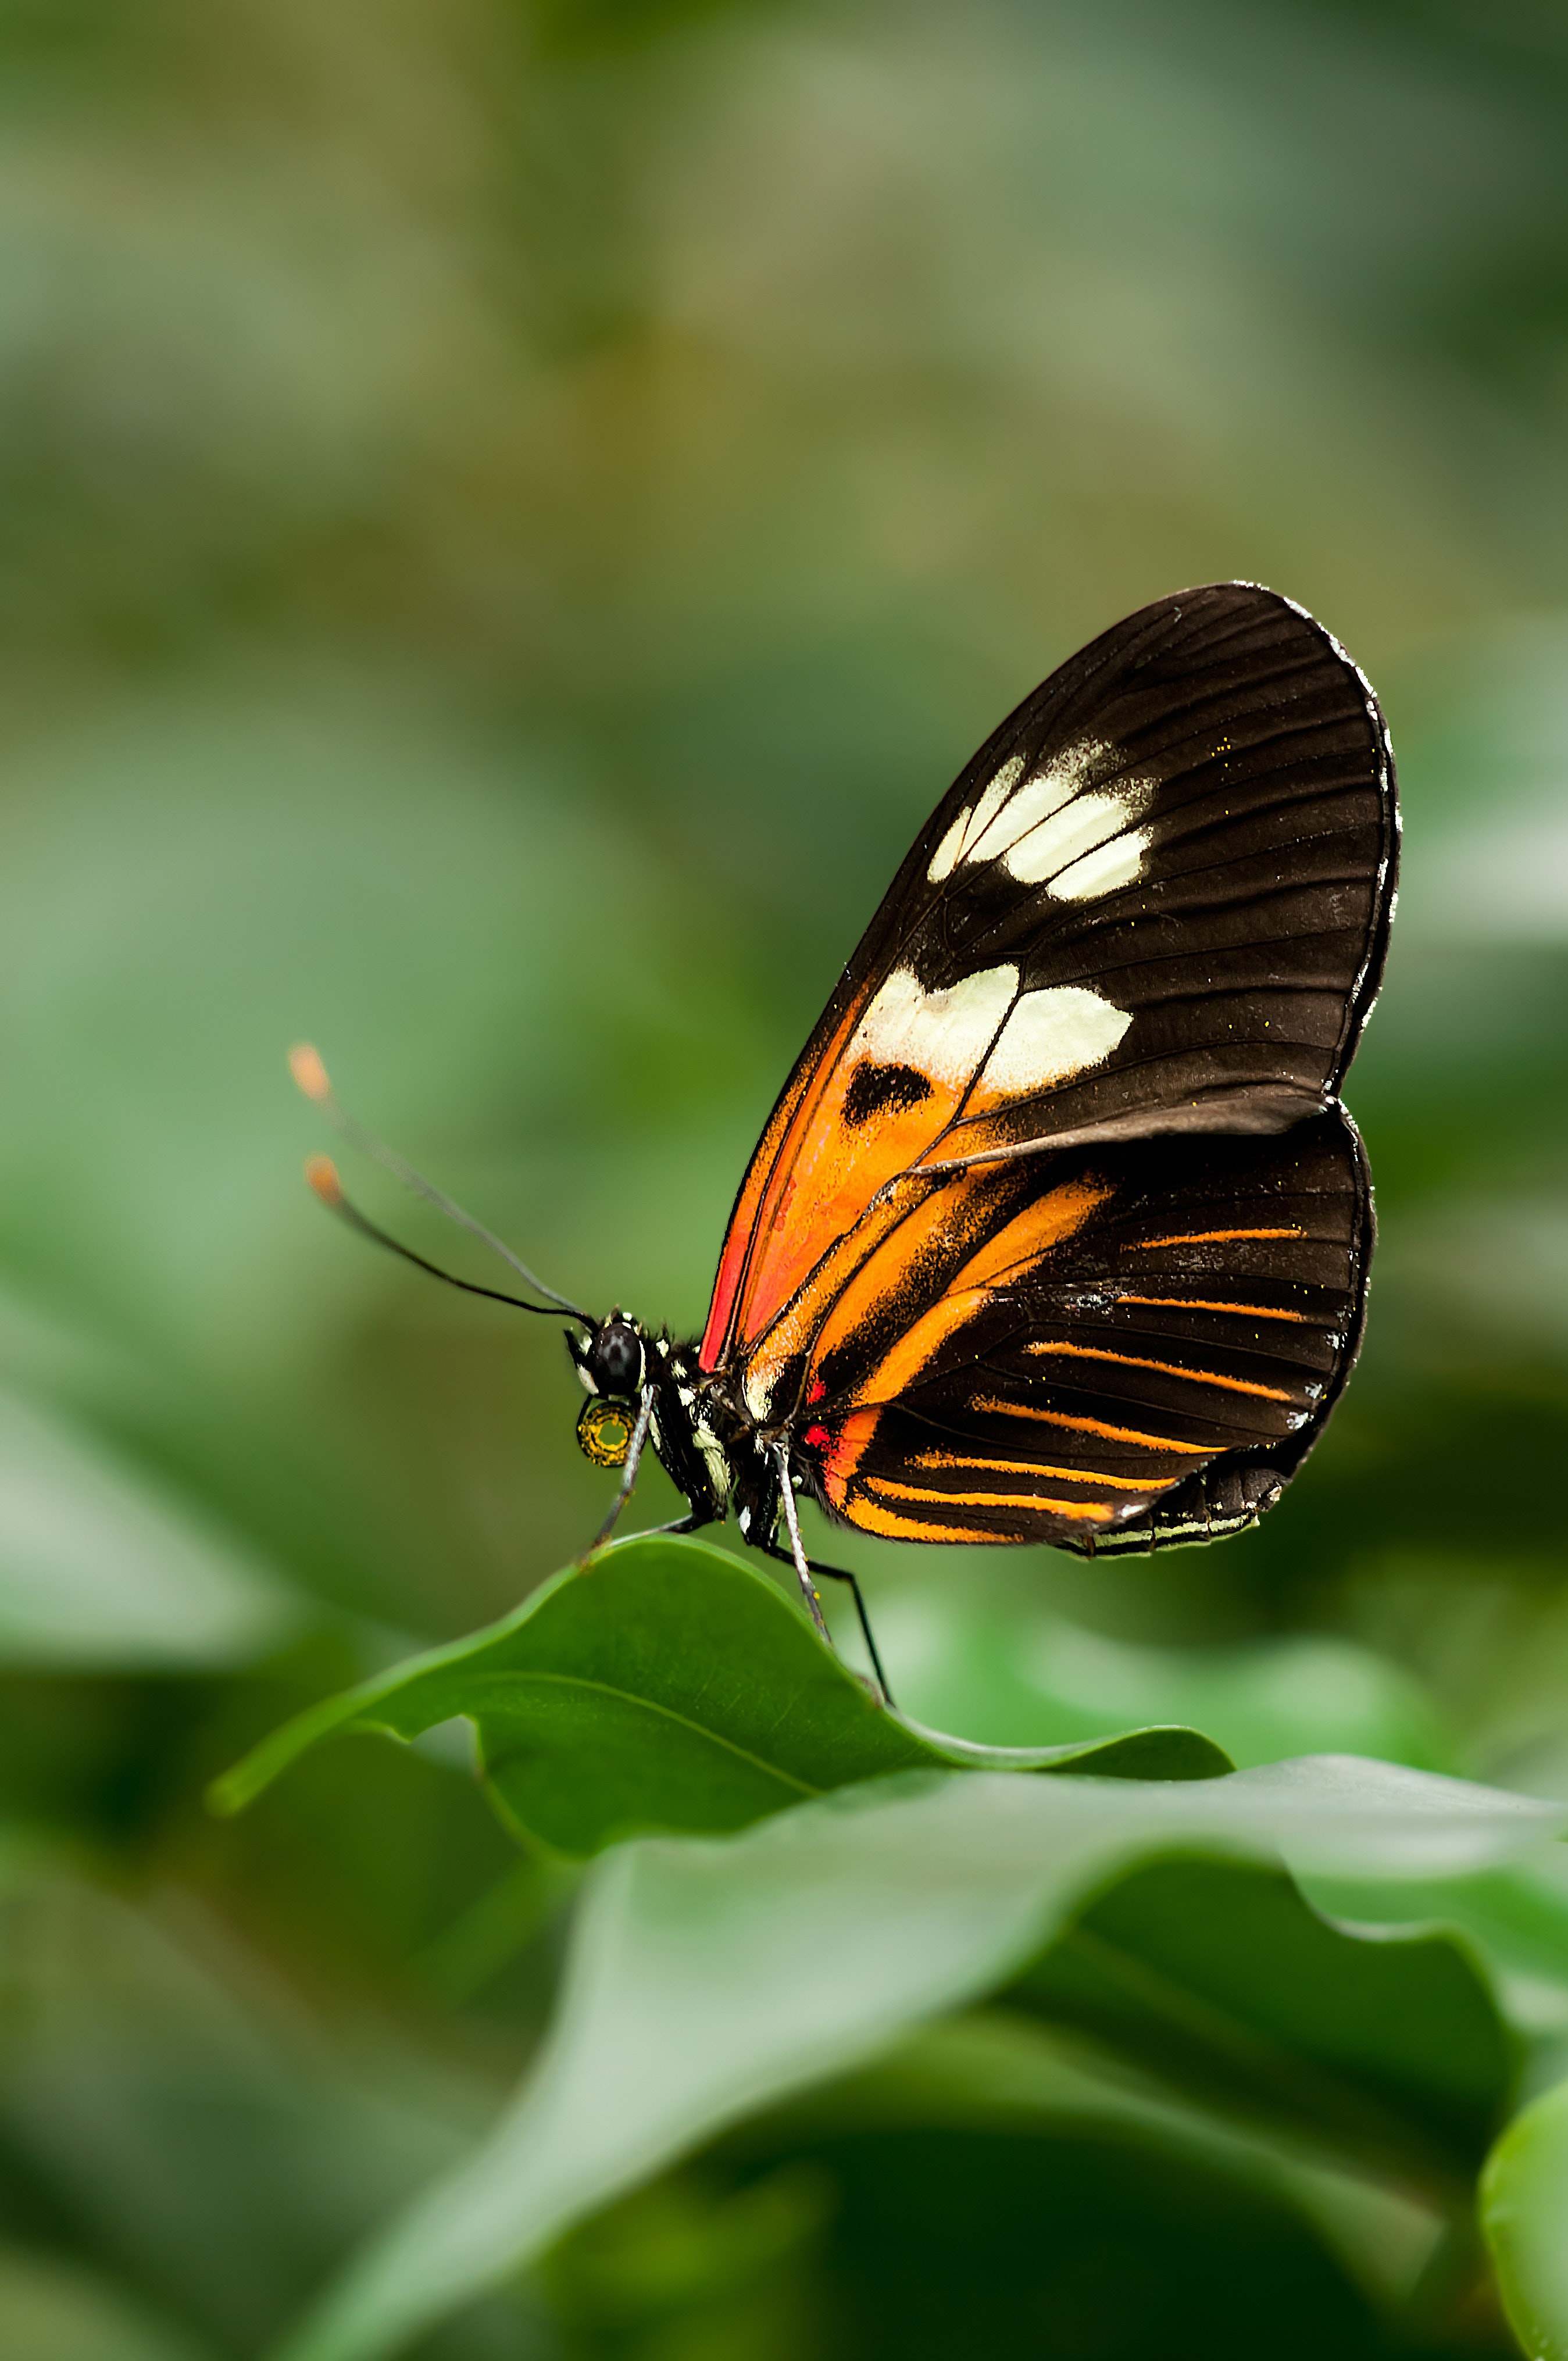
\includegraphics[width=4cm,height=4cm]{butterfly1.jpg}
\caption{butterfly figure 1}
\label{fig:butterfly1}
\end{figure}
\end{column}
\end{columns}
\end{frame}
\begin{frame}{Wrapping figure around text}
\begin{wrapfigure}{l}{0.5\textwidth}
	% l for left and r right
	\centering
	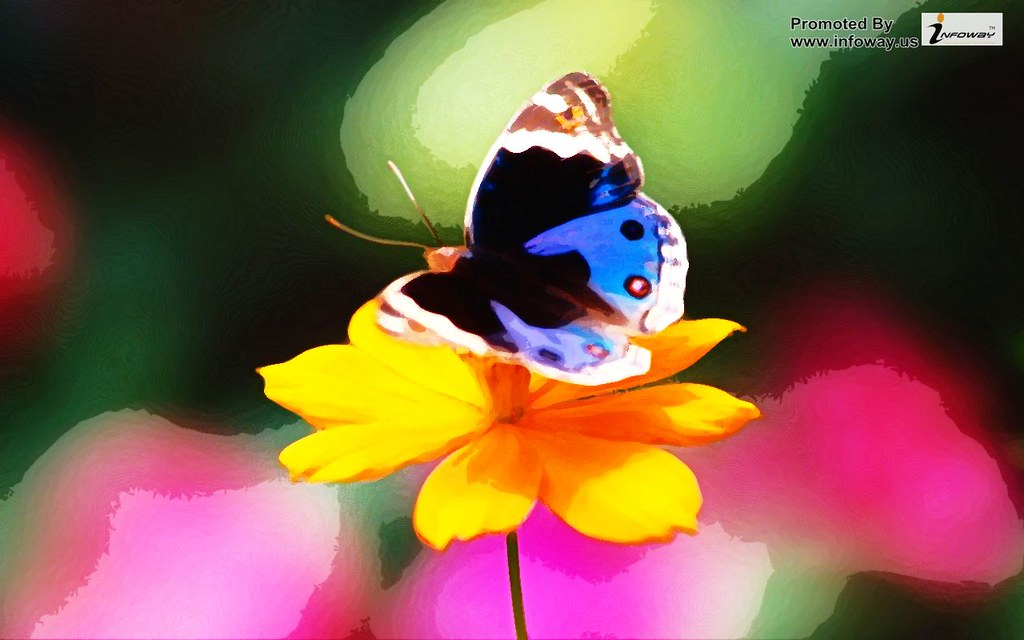
\includegraphics[width=0.4\textwidth]{butterfly2.jpg}
	\caption{wrapping figure around text}
\end{wrapfigure}
\small\blindtext	
\end{frame}
\begin{frame}{text over image}
\begin{tikzpicture}
	\node(image)
	{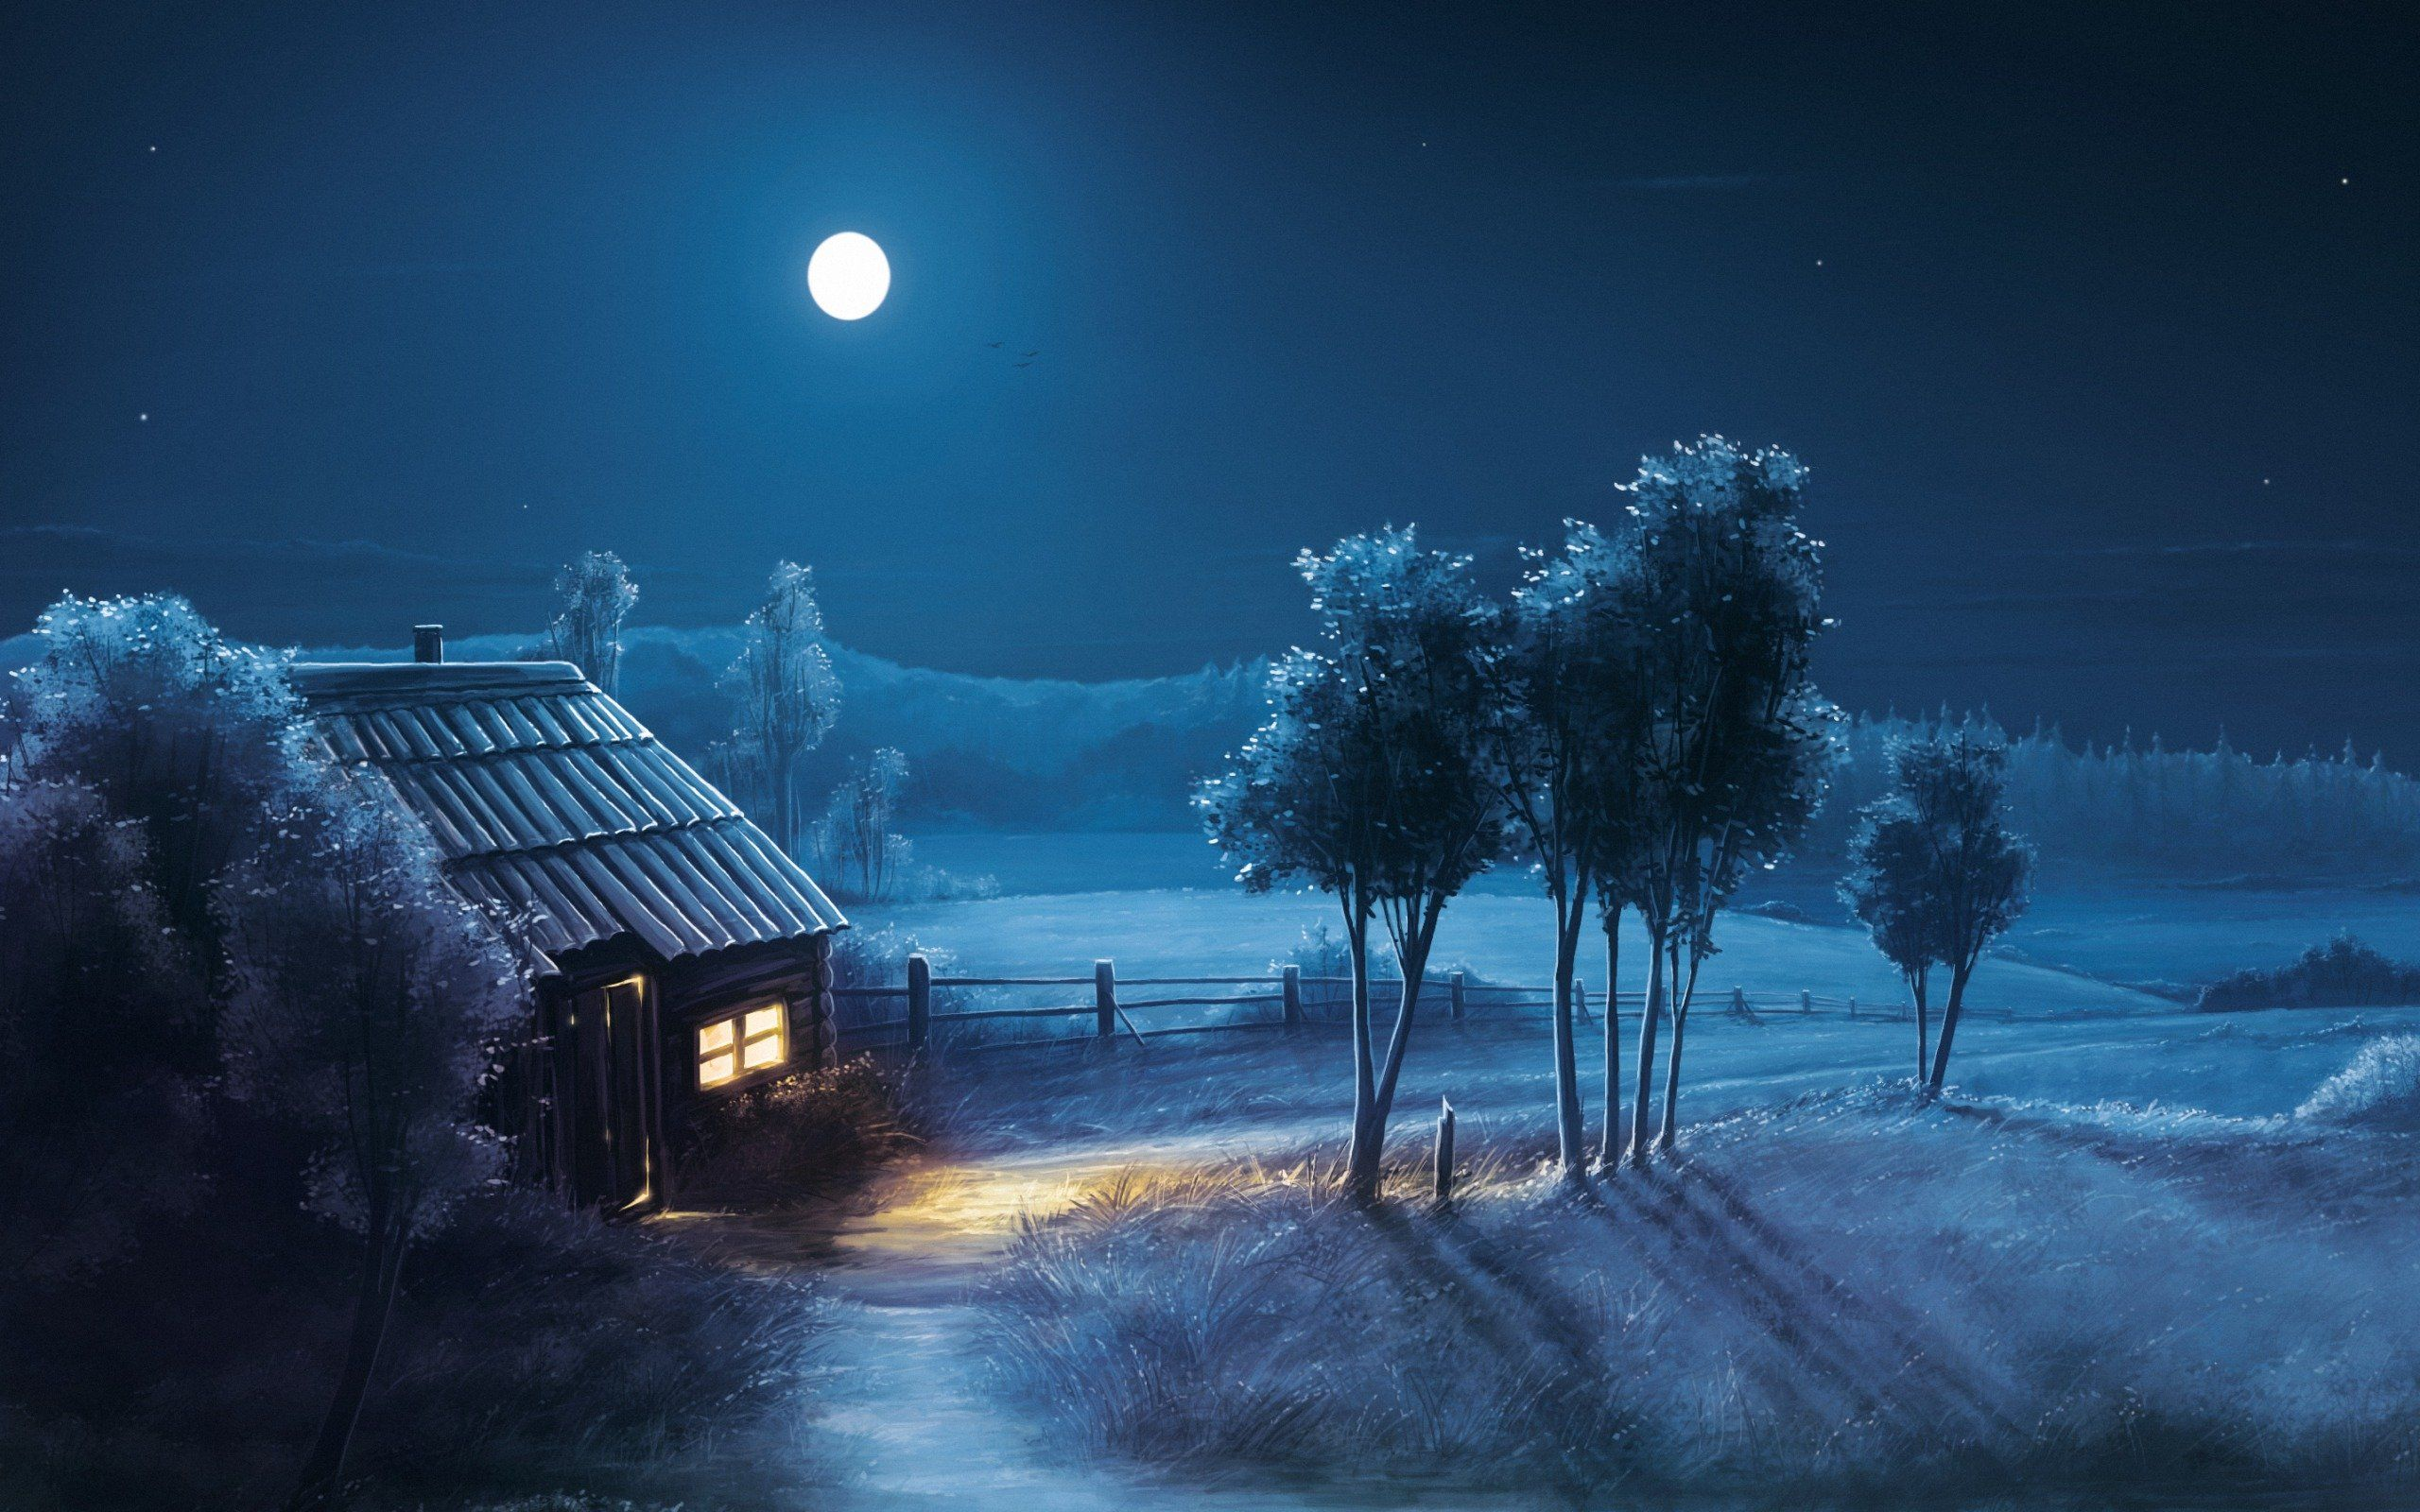
\includegraphics[width=1\textwidth]{night1.jpg}};
	\node
	[
	fill=teal,
	align=center,
	text=white,
	font={\huge\bfseries}
	]at (image.center){A beautiful Night!};
\end{tikzpicture}
\end{frame}
\begin{frame}{Subfigure in Beamer}
	\begin{figure}[h]
		\begin{subfigure}[t]{0.4\textwidth}
			\centering
		
\includegraphics[width=0.5\linewidth]{butterfly3.jpg}
		\caption{Butterfly figure 3}
		\label{fig:butterfly3}
		\end{subfigure}
	\begin{subfigure}[b]{0.4\textwidth}
		\centering
		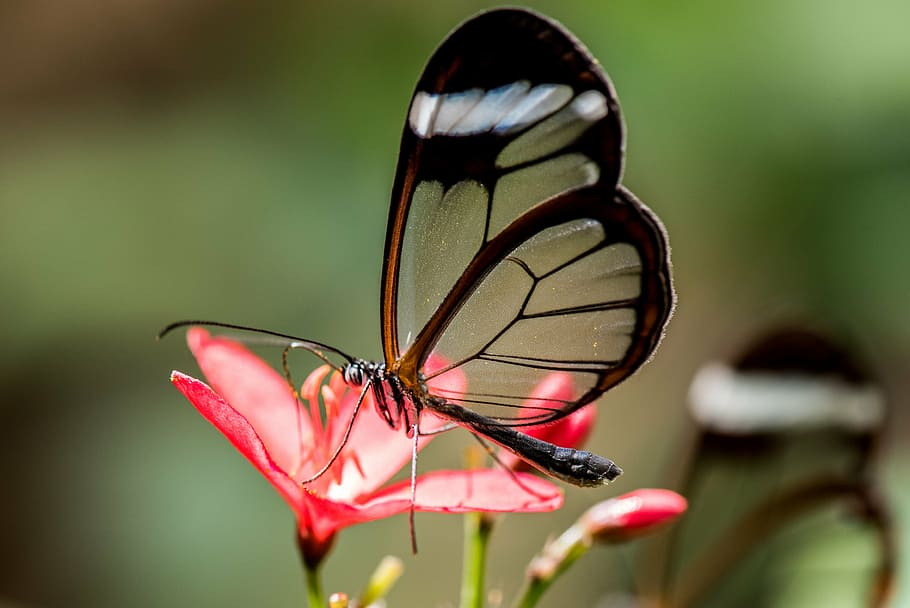
\includegraphics[width=0.5\linewidth]{butterfly4.jpg}
		\caption{butterfly4}
		\label{fig:butterfly4}	
	\end{subfigure}
\caption{subfigure}
\label{fig:image}
	\end{figure}
\end{frame}
\begin{frame}{animations:animate with text using pause}
	first line will appear in this slide\\ \pause
	the second text will be partially visible\\ \pause
	and this last text will appear
\end{frame}
\begin{frame}{animation in the itemize:overlay specification}
	\begin{itemize}
		\item<1-> item 1
		\item<2-> item 2
		\item<3-> item 3
	\end{itemize}
	
\end{frame}
\end{document}
%==========================================================%
% Commented Templete 
%==========================================================%
%-----------+-----------------+------------------%
% Frame for the columns
%**********************%
%\begin{frame}{Columns}
%% columns with top allignment use [T], for center alignment[c],for bottom alignment[b]
%\begin{columns}[T]
%	%column 1
%	\begin{column}{0.49\linewidth}
	%	\small	\blindtext
	%	\end{column}
%%column for the verticle length
%\begin{column}{0.01\linewidth}
%	\rule{0.1mm}{0.7\textheight}
%\end{column}
%% column 2
%	\begin{column}{0.49\linewidth}
	%		\small	\blindtext
	%	\end{column}
%\end{columns}
%\end{frame}
%---------+--------------------+-----------------%
% Frame for the Blocks
%*********************%
%\begin{frame}{Blocks}
% Generic and standard Block
%	\begin{block}{Block title}
	%		block 1
	%	\end{block}
%Block for the definition
%\begin{definition}
%	definition
%\end{definition}
%\end{frame}
%---------+-------------------+------------------%
% Frame for making table
%*********************%
%\begin{frame}{wraptable}
%\begin{wraptable}{r}{0.5\textwidth}
%\centering
%\begin{tabular}{|c|c|c|} 
%		\hline
%		1&2& 3 \\
%		\hline
%		4&5&6\\
%		\hline
%	\end{tabular}
%\caption{ Table template}
%\label{tab:table}
%\end{wraptable}
%\blindtext
%\end{frame}
%---------+---------------------+----------------%
% Frame for text box
%********************%
%\begin{frame}{text Boxes}
%\shadowbox{Text}\\	
%\fbox{text}	\\
%\doublebox{text}\\
%\ovalbox{text}\\
%\end{frame}
%---------+---------------------+----------------%
% Frame for list of ding
%***********************%
%\begin{frame}{Lists in Beamer}
%\begin{itemize}
%	\item[\ding{51}] code 51 
%	\item[\ding{56}] code 56
%	\item[\ding{43}] code 43
%	\item[\ding{45}] code 45
%	\item[\ding{79}] code 79
%	\item[\ding{118}] code 118
%\end{itemize}
%-----------------
%\begin{itemize}
%	\item[\ding{118}] code 118
%\end{itemize}
%--------------------------
%\end{frame}
%---------+----------------------+---------------%
% Templete to include graphics
%******************************%
%	\begin{figure}[t]
%		\centering
%		\includegraphics[width=0.6\linewidth]{slide3fig1(BZ).pdf}
%	\end{figure}
%---------+----------------------+---------------%
% Templete to include fbox
%\centering
%\fbox{\parbox{0.7\linewidth}{\textcolor{magenta}{}}
%}
%---------+----------------------+---------------%
%\usepackage{derivative}
% Beamer theme
%\usetheme{Singapore}
%\usecolortheme{rainbow}
% Font theme
% Font theme
%\usefonttheme{structuresmallcapsserif}
% Set color in the theme
%==================color theme========================%
%\definecolor{fgblack}{rgb}{0.0,0.65,0.58}
%\usecolortheme[named=fgblack]{structure}
%==========================================%
%\setbeamercolor{title}{bg=bgcolor}
%\setbeamercolor{Frametitle}{bg=bgcolor}
%\setbeamercolor{structure}{bg=bgcolor}
% Frame size
%\setbeamersize{text margin left=1mm,text margin right=1mm}
%==================customization of Block=======================%
%\setbeamertemplate{block}[rounded]
%\definecolor{black}{rgb}{0.0,0.0,0.0}
%\definecolor{turgreen}{rgb}{0.59,0.87,0.82}
%\setbeamercolor{block title}{bg=turgreen, fg=black}
%\setbeamercolor{block body}{bg=cyan!10}